\documentclass[
	12pt,				% tamanho da fonte		
	oneside,
	a4paper,			% tamanho do papel.
	chapter=TITLE,
	%sumario=tradicional,
	brazil,				% idioma adicional
	english,			% idioma principal do documento
	]{abntex2}

% ---
% PACOTES
% ---
\usepackage{lmodern}			% Usa a fonte Latin Modern
\usepackage[T1]{fontenc}		% Selecao de codigos de fonte.
\usepackage[utf8]{inputenc}		% Codificacao do documento (conversão automática dos acentos)
\usepackage{indentfirst}		% Indenta o primeiro parágrafo de cada seção.
\usepackage{color}				% Controle das cores
\usepackage{graphicx}			% Inclusão de gráficos
\graphicspath{{figuras/},{figuras/Intro/},{figuras/CAP2/},{figuras/CAP3/},{figuras/CAP4/},{figuras/CAP5/}}
\usepackage{microtype} 			% para melhorias de justificação
\usepackage{booktabs}
\usepackage{float} 				% Set posição da figura
\usepackage[bottom]{footmisc} 
\usepackage{subfig} 			% Inserir subfiguras
\usepackage[table,xcdraw]{xcolor} 	% Cor de preenchimento das tabelas
\usepackage{multirow} 			%mesclar cel em tabelas
\usepackage{verbatim}			%Inserir codigos fontes e comentários em massa
\usepackage[alf]{lib/abntex2cite}
\usepackage[brazilian,hyperpageref]{backref}
\usepackage{lipsum}				% para geração de dummy text
\usepackage{amsmath}
\usepackage[bottom]{footmisc}
\usepackage{footnote}
% Para incluir pseudocódigos
\usepackage[portuguese, ruled, linesnumbered]{algorithm2e}
%\usepackage{fnpos}
%\usepackage{ftnxtra}
\usepackage{listings} 			%Inserir códigos fontes
\usepackage{rotating} 			%Rotação de páginas
\usepackage{placeins}			% Forçar o posicionamento da figura
\usepackage[top=3cm, bottom=2cm, left=3cm, right=2cm]{geometry} % Margens

% ---
% Informações de dados para CAPA e FOLHA DE ROSTO
% ---

\titulo{{\normalfont \textbf{NECTA: Neural Connectivity Time-resolved Analysis}}}
\autor{Jaime Bruno Cirne de Oliveira}
\local{Natal -- Rio Grande do Norte, Brazil}
\data{2026}
\instituicao{
 % Universidade Federal do Rio Grande do Norte -- UFRN
 % \par
 % PROGRAMA DE PÓS-GRADUAÇÃO EM BIOINFORMÁTICA -- Biome
 % \par
 % DOUTORADO EM BIOINFORMÁTICA
}
\tipotrabalho{Thesis (Doctoral)}

\preambulo{Thesis presented to the Graduate Program in
Bioinformatics at
the Federal University of Rio Grande do Norte in
partial fulfillment of the requirements for obtaining
the degree of Doctor in Bioinformatic
\newline 
\newline 
Advisor: Prof. Drª. Kerstin Erika Schmidt}

% Configurações de aparência do PDF final
% alterando o aspecto da cor azul
\definecolor{blue}{RGB}{41,5,195}
% informações do PDF
\makeatletter
\hypersetup{
     	%pagebackref=true,
		pdftitle={\@title}, 
		pdfauthor={\@author},
    	pdfsubject={\imprimirpreambulo},
	    pdfcreator={LaTeX with abnTeX2},
		pdfkeywords={abnt}{latex}{abntex}{abntex2}{relatório técnico}, 
		colorlinks=true,       		% false: boxed links; true: colored links
    	linkcolor=black,          	% color of internal links
    	citecolor=black,        		% color of links to bibliography
    	filecolor=magenta,      		% color of file links
		urlcolor=blue,
		bookmarksdepth=4
}

\makeatother
% Espaçamentos entre linhas e parágrafos 
\setlength{\parindent}{1.25cm} % Tamanho do parágrafo
\setlength{\parskip}{0.2cm}	% Controle do espaçamento entre um parágrafo e outro

%\onelineskip % Controle do espaçamento entre um parágrafo e outro

\makeindex % compila o indice

% Início do documento
% ----
\begin{document}

% Seleciona o idioma do documento (conforme pacotes do babel)
\selectlanguage{english}
%\selectlanguage{brazil}

% Retira espaço extra obsoleto entre as frases.
\frenchspacing 

% ----------------------------------------------------------
% ELEMENTOS PRÉ-TEXTUAIS
% ----------------------------------------------------------
\pretextual

% Capa
\imprimircapa

% Folha de rosto
\imprimirfolhaderosto

% Inserir folha de aprovação
\begin{folhadeaprovacao}
	
	\begin{center}
		{\ABNTEXchapterfont\large\imprimirautor}
		
		\vspace*{\fill}\vspace*{\fill}
		\begin{center}
			\ABNTEXchapterfont\bfseries\Large\imprimirtitulo
		\end{center}
		\vspace*{\fill}
		
		\hspace{.45\textwidth}
		\begin{minipage}{.5\textwidth}
			\imprimirpreambulo
		\end{minipage}%
		\vspace*{\fill}
	\end{center}
	
	\imprimirlocal, x June 2026, Defense Committee:
	
	
	\setlength{\ABNTEXsignwidth}{14cm}
	\assinatura{\textbf{Prof. Drª Kerstin Erika Schmidt - Advisor} \\ UFRN} 
	\assinatura{\textbf{Prof. Dr. Daniel Yasumasa Takahashi - } \\ UFRN}
	\assinatura{\textbf{Prof. Dr. Patrick Cesar Alves Terrematte - } \\ UFRN }
	
	\begin{center}
		\vspace*{0.5cm}
		{\large\imprimirlocal}
		\par
		{\large\imprimirdata}
		\vspace*{1cm}
	\end{center}
	
\end{folhadeaprovacao}

% Dedicatória
\begin{dedicatoria}
	\vspace*{\fill}
	\centering
	\noindent
	\textit{}
	 \vspace*{\fill}
\end{dedicatoria}

% Agradecimentos
\begin{agradecimentos}
To my advisor, Prof. Dr. Kerstin Erika Schmidt, I express my deepest gratitude for the opportunity to pursue this PhD, as well as for her continuous dedication and care for me and my research. Her work and academic posture serve as a true inspiration for my future horizon.

To my colleagues, with a special thanks to Gabriel Marcos da Silva, Israel Araújo do Nascimento Dantas, and Daniel Walmir dos Santos Alves, for the immense support that allowed me to balance my academic and professional life in such a challenging context. Still in this scenario, I thank Juliana Alves Brandão Medeiros de Sousa who, like me, walked this academic and professional path at the Brain Institute, sharing valuable insights that made this journey possible.

To the professors of the Graduate Programs in Bioinformatics (PPG-BioInfo) and Neurosciences (PPG-Neuro) who directly contributed to my academic formation and research, especially Daniel Yasumasa Takahashi and Sergio Neuenschwander.

To Friedrich Schwarz, I leave a special thanks for providing fundamental insights that guided the direction of this work. I am also grateful to him for providing the VisualICeIO project, which enabled the analysis of the laboratory's data and allowed me to focus more deeply on the analyses of NECTA.

Finally, the most essential and affectionate thanks go to my family. To my parents, Mauro Borges de Oliveira and Marizeth Cirne de Oliveira, who had the greatest and most definitive impact on the person I am today. To my live-in partner, Ingrid Bárbara Ramos Ho, with whom I share my life and who, so many times, provided the environment of stability, love, and support that was vital for the realization of this work.
\end{agradecimentos}

% ---
% Epígrafe
% ---
\begin{epigrafe}
	\vspace*{\fill}
	\begin{flushright}
		\textit{``It pays to keep an open mind, but not so open your brains fall out."\\
			(Carl Sagan)}
	\end{flushright}
\end{epigrafe}

% RESUMO
% resumo na língua vernácula (obrigatório)
\setlength{\absparsep}{18pt} % ajusta o espaçamento dos parágrafos do resumo
\begin{resumo}[Resumo]

A análise tradicional da conectividade funcional do cérebro frequentemente colapsa a dimensão temporal, gerando grafos estáticos que mascaram a evolução dinâmica das redes neurais, o chamado "Dinoma" (Dynome). Além disso, a extração de redes resolvidas no tempo a partir de dados de eletrofisiologia de alta densidade (LFP) esbarra no fenômeno físico da condução de volume e no gargalo computacional associado ao processamento estocástico de Big Data. Esta tese de qualificação apresenta o NECTA (Neural Connectivity Time-resolved Analysis), um framework computacional interativo de alto desempenho projetado para a exploração metodológica do mesoconectoma dinâmico. O NECTA emprega uma arquitetura paralela baseada em Dask e armazenamento otimizado nativo de nuvem em Zarr para orquestrar simulações estocásticas em larga escala, fatiamento de tensores multidimensionais e modelos nulos topológicos, superando de maneira linear as limitações críticas de memória RAM (Out-Of-Memory) de fluxos analíticos tradicionais. O framework mitiga ativamente os artefatos de condução volumétrica (zero-phase lag) através de processamentos no sinal analítico de Hilbert, utilizando estimadores complexos baseados em fase, como o Índice de Atraso de Fase Ponderado (wPLI) e a Coerência Imaginária (iCoh). Para inferência causal estrita, implementou-se a Coerência Direcionada Parcial (PDC) em um módulo auto-otimizado dinamicamente pelo Critério de Informação Bayesiana (BIC), controlando penalizações de complexidade em regressões autorregressivas vetoriais (MVAR). O sistema foi validado in silico (contra ruído sintético e condução modelada) e aplicado empiricamente a um dataset de 48 canais do córtex visual primário felino (Área 17, Área 18 e Zona de Transição), registrado sob anestesia geral e paralisia (isolando oscilações intrínsecas de modulações cognitivas atencionais). Os resultados in vivo demonstraram que o córtex visual exibe intensas e ativas flutuações topológicas de alta frequência, atingindo picos transientes de eficiência de "Mundo Pequeno" (Small-Worldness) precisamente coordenados durante a estimulação visual por grades em movimento. A análise direcional na banda Low Gamma (30-59 Hz) estabeleceu a Área 17 como um nó Fonte (Driver) persistente e a Área 18 como um Sumidouro (Sink) estável, enquanto a Zona de Transição atuou como um robusto modulador dinâmico do fluxo inter-hemisférico, alternando sua direcionalidade causal sob estimulação. O NECTA democratiza análises avançadas em neuroinformática, entregando um ecossistema interativo (Dash/Cytoscape) reprodutível focado em Open Science que habilita a tradução ágil e sistêmica de sinais eletrofisiológicos brutos em descobertas conectômicas cronológicas.

\vspace{\onelineskip}
 \noindent
 \textbf{Palavras-chaves}: Conectividade Funcional Dinâmica; Eletrofisiologia; Computação de Alto Desempenho; Coerência Direcionada Parcial; Córtex Visual.
\end{resumo}

% ---
% resumo em inglês
\begin{resumo}[Abstract]
	\begin{otherlanguage*}{english}
	
	Traditional analysis of brain functional connectivity often collapses the temporal dimension, generating static graphs that obscure the dynamic evolution of neural networks, known as the "Dynome". Furthermore, extracting time-resolved networks from high-density electrophysiology (LFP) is heavily hindered by the physical phenomenon of volume conduction and the computational bottleneck associated with stochastic Big Data processing. This qualifying thesis presents NECTA (Neural Connectivity Time-resolved Analysis), an interactive high-performance computational framework designed to explore the dynamic mesoconnectome. NECTA employs a Dask-based parallel architecture and cloud-native Zarr-optimized storage to orchestrate large-scale stochastic simulations, multidimensional tensor slicing, and topological null models, linearly overcoming the critical RAM (Out-Of-Memory) limitations of traditional analytical pipelines. The framework actively mitigates volume conduction artifacts (zero-phase lag) through Hilbert analytical signal processing, utilizing phase-based complex estimators such as the Weighted Phase Lag Index (wPLI) and Imaginary Coherence (iCoh). For strict causal inference, Partial Directed Coherence (PDC) was implemented within a module dynamically auto-optimized by the Bayesian Information Criterion (BIC), controlling complexity penalties in multivariate autoregressive regressions (MVAR). The system was validated in silico (against synthetic noise and modeled conduction) and empirically applied to a 48-channel dataset from the feline primary visual cortex (Area 17, Area 18, and the Transition Zone), recorded under general anesthesia and paralysis (isolating intrinsic oscillations from top-down cognitive modulations). In vivo results demonstrated that the visual cortex exhibits intense and active high-frequency topological fluctuations, reaching transient peaks in Small-Worldness efficiency precisely coordinated during visual stimulation by moving gratings. Directed analysis in the Low Gamma band (30-59 Hz) established Area 17 as a persistent Driver node (Source) and Area 18 as a stable Sink, while the Transition Zone acted as a robust dynamic modulator of interhemispheric flow, alternating its causal directionality upon stimulation. NECTA democratizes advanced neuroinformatics analyses, delivering a reproducible, Open Science-oriented interactive ecosystem (Dash/Cytoscape) that enables the agile and systemic translation of raw electrophysiological signals into chronological connectomic discoveries.
	
	\vspace{\onelineskip}
	\noindent 
	\textbf{Keywords}: Dynamic Functional Connectivity; Electrophysiology; High-Performance Computing; Partial Directed Coherence; Visual Cortex.
	\end{otherlanguage*}
\end{resumo}

% ---
% inserir lista de ilustrações
\pdfbookmark[0]{\listfigurename}{lof}
\listoffigures*
\cleardoublepage

% inserir lista de tabelas
\pdfbookmark[0]{\listtablename}{lot}
\listoftables*
\cleardoublepage

% inserir lista de abreviaturas e siglas
\begin{siglas}
\item[HTML] \textit{HyperText Markup Language}
\item[JSON] \textit{JavaScript Object Notation}
\item[REST] \textit{Representational State Transfer}
\end{siglas}

% inserir lista de símbolos
\begin{simbolos}
  \item[$ \Gamma $] Letra grega Gama
  \item[$ \Lambda $] Lambda
  \item[$ \zeta $] Letra grega minúscula zeta
  \item[$ \in $] Pertence
\end{simbolos}

% inserir o sumario
\pdfbookmark[0]{\contentsname}{toc}
\tableofcontents*
\cleardoublepage

\textual

% Capitulo 1: Introdução
\chapter{INTRODUCTION}

\subsection{The Primary Visual Cortex and the Limits of Static Topologies}
The primary visual cortex has long served as the canonical model for understanding cortical microcircuitry, sensory processing, and the brain's \textbf{neural networks}. Historically, the architectural and functional parcellation of visual areas---such as Area 17 (A17), Area 18 (A18), and their Transition Zone (TZ) in the feline model---has been extensively mapped using single-unit recordings and static receptive field analyses (Wunderle et al., 2013; Schmidt et al., 2023). These classical approaches have established the foundational \textbf{static connectome}---a rigid, structural blueprint of the visual system detailing how intra- and inter-hemispheric neural networks form clustered functional communities. 
\begin{figure}[htbp]
    \centering
    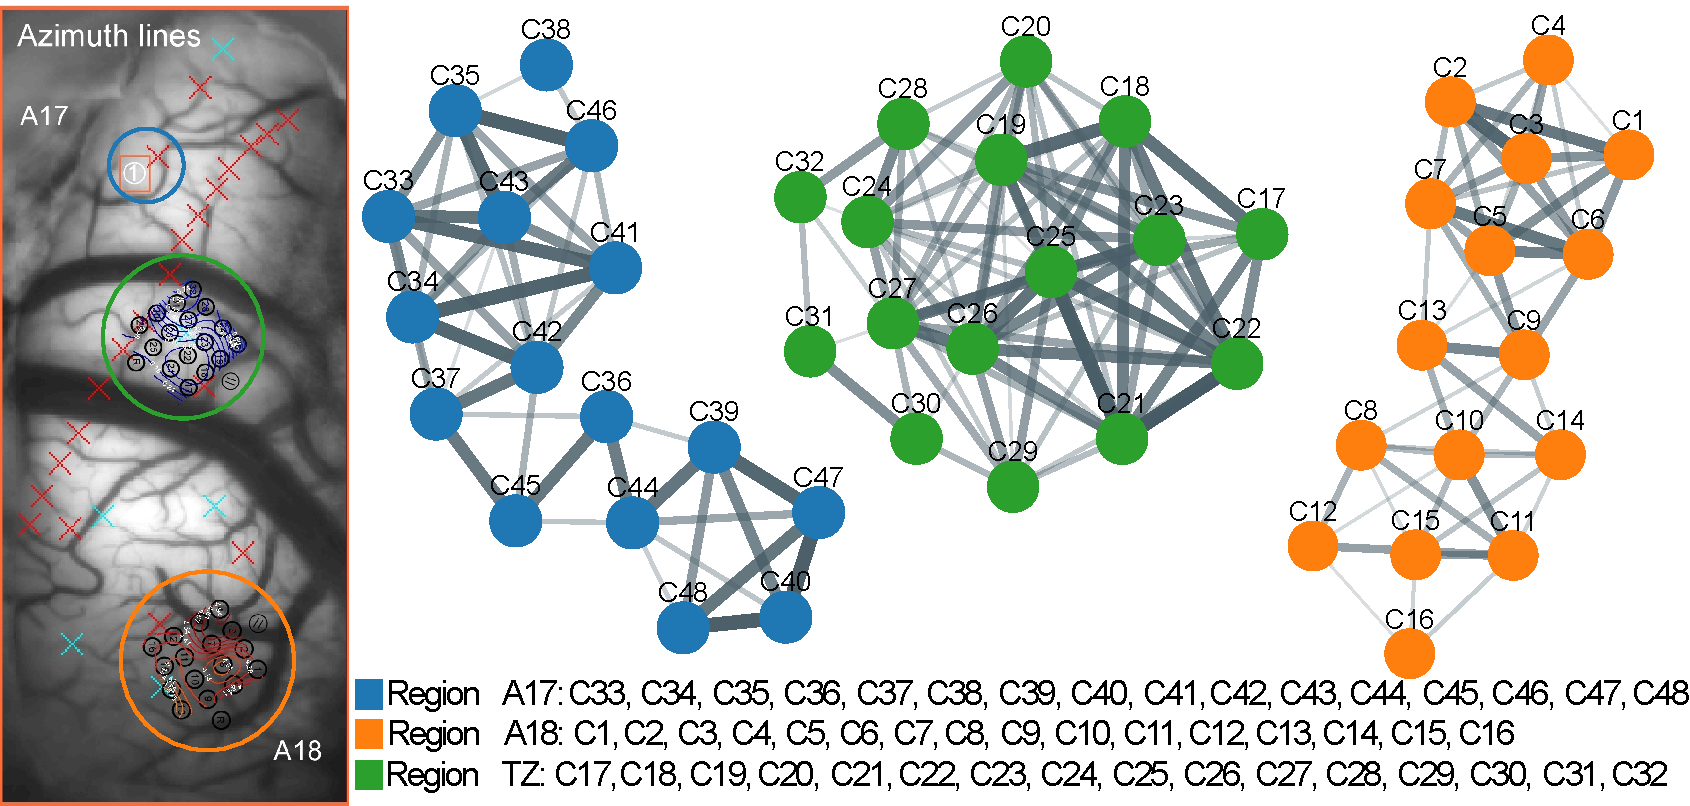
\includegraphics[width=\linewidth]{./figuras/Intro/Figura01.pdf}
    \caption[Mapping directly to the anatomically separated electrode matrixes]{\textbf{Mapping directly to the anatomically separated electrode matrixes | (Coherence (Low Gamma)) | Density: 15\%: Coherence clusters}}
    \label{fig:cortical_model}
\end{figure}
However, relying exclusively on these stationary statistical relationships collapses the true, living matrix of cortical connections. Averaging neural interactions over long temporal windows (e.g., minutes of recording) treats the neural network as a fixed roadmap, inevitably obscuring sub-second synaptic recruitment and leading to a severe loss of organic causality resolution. Cognitive processes, particularly visual feature binding, do not operate in a stationary state; they evolve dynamically and transiently as stimuli move across and between receptive fields. Consequently, \textbf{static topologies}---while accurately describing the anatomical constraints and the baseline connectome of neural communication---completely mask the rapid, transient fluctuations in functional integration that are the actual hallmark of active sensory processing.


\section{The Paradigm Shift to the "Dynome"}
To overcome the limitations of static connectomics, the neuroscientific community has begun shifting its focus toward the exploration of the "Dynome"—the millisecond-scale evolution of functional networks and their temporal dynamics \cite{kopell2014}. Capturing the Dynome requires shifting the analytical framework from time-averaged correlations to time-resolved state transitions, often achieved through sliding-window approaches \cite{allen2014}. By dissecting the continuous data stream into granular temporal epochs, it becomes possible to observe how network metrics, such as \textit{Small-Worldness} and modularity, adapt and evolve. This time-varying perspective provides a much more accurate representation of the brain's real-time functional state, revealing that macroscopic efficiency is not fixed but reacts continuously to ongoing sensory integration.

\section{Rhythmic Oscillations, Predictive Coding, and Gamma Synchronization}
At the mesoscopic scale, rhythmic neural oscillations—specifically in the Gamma frequency band (30–90 Hz)—act as a fundamental mechanism for cortical communication and information routing. Under the predictive coding framework, the synchronized engagement of neuronal populations in the gamma band provides a fast transmission channel for feedforward visual processing, carrying sensory "prediction errors" from primary areas (A17) to higher-order regions (A18) \cite{vezoli2021}. Furthermore, the Transition Zone (TZ) acts not merely as a geographic boundary, but as a highly specialized region densely innervated by transcallosal projections, facilitating massive interhemispheric coordination essential for integrating visual stimuli across the vertical meridian \cite{schmidt2023}. Thus, mapping the directionality of gamma synchronization across A17, TZ, and A18 is crucial for deciphering the causal architecture and dynamic modulation of the visual cortex.

\section{The Methodological Bottleneck in Electrophysiology}
Despite the theoretical necessity of time-resolved, directed connectivity analysis, extracting these networks from dense multi-electrode arrays poses severe methodological and computational challenges. The primary analytical bottleneck in Local Field Potential (LFP) analysis is \textit{volume conduction}—the instantaneous spread of electrical fields through cortical tissue. This phenomenon causes multiple electrodes to record a single biological source simultaneously, generating spurious zero-phase lag correlations that heavily contaminate graph topologies with false-positive edges \cite{bastos2015}.

Furthermore, the transition to high-density electrophysiology (e.g., 32-64 channel matrices) creates a "Big Data" computational crisis. Calculating dynamic, non-linear connectivity metrics (such as Partial Directed Coherence or phase-based indices), generating hundreds of surrogate networks for statistical validation, and tracking graph properties over moving time windows inevitably lead to combinatorial explosions. Traditional, single-threaded analytical scripts are inherently incapable of managing such stochastic, multidimensional loads, often resulting in Out-of-Memory (OOM) failures or prohibitive processing times. 

Consequently, there is a critical need for a modern, high-performance computing (HPC) framework capable of mitigating volume conduction artifacts through advanced phase-based estimators while leveraging distributed parallel processing to interactively render the mesoscopic Dynome.

\vspace{1cm}

% --- VISUAL INSERTION USING TIKZ ---
\begin{figure}[htbp]
    \centering
    \begin{tikzpicture}[
        box/.style={draw, rounded corners, minimum width=2.5cm, minimum height=1cm, align=center, fill=blue!5, font=\sffamily\small},
        circ/.style={draw, circle, minimum size=1.5cm, align=center, fill=red!5, font=\sffamily\small},
        >={Stealth},
        thick
    ]
        
        % ================= PANEL A =================
        \node[font=\bfseries\sffamily] at (0, 0) {Painel A: Condução de Volume vs. Resolução Analítica};
        
        % Volume Conduction Side
        \node[circ] (dipole) at (-4, -2) {Deep\\Dipole};
        \node[box] (e1) at (-7, -5) {CH 1};
        \node[box] (e2) at (-4.5, -5) {CH 2};
        \node[box] (e3) at (-2, -5) {CH 3};
        \node[box] (e4) at (0.5, -5) {CH 4};
        
        \draw[->, dashed] (dipole) -- (e1);
        \draw[->, dashed] (dipole) -- (e2);
        \draw[->, dashed] (dipole) -- (e3);
        \draw[->, dashed] (dipole) -- (e4);
        
        \draw[<->, red] (e1) to[bend right=25] node[below, font=\scriptsize\sffamily] {Zero-lag} (e2);
        \draw[<->, red] (e2) to[bend right=25] (e3);
        \draw[<->, red] (e3) to[bend right=25] (e4);
        \draw[<->, red] (e1) to[bend right=40] (e4);
        
        % Filter Side
        \node[box, fill=orange!10, minimum height=1.5cm] (filter) at (4, -2.5) {Complex Domain\\Filter\\(wPLI / iCoh)};
        
        \node[circ, fill=green!10] (n1) at (2.5, -5) {Node 1};
        \node[circ, fill=green!10] (n3) at (5.5, -5) {Node 3};
        
        \draw[->, ultra thick] (e4.east) to[out=0, in=180] (filter.west);
        \draw[->, ultra thick] (filter.south) -- (4, -3.8) -| (n1.north);
        \draw[->, ultra thick] (filter.south) -- (4, -3.8) -| (n3.north);
        
        \draw[<->, ultra thick, green!50!black] (n1) -- node[above, font=\scriptsize\sffamily] {Valid Edge} (n3);
        
        
        % ================= PANEL B =================
        \node[font=\bfseries\sffamily] at (0, -8.5) {Painel B: Colapso Temporal vs. Dinoma Transiente};
        
        % Static Approach
        \node[box] (t1) at (-5.5, -10) {State 1};
        \node[box] (t2) at (-2.5, -10) {State 2};
        \node[box] (t3) at (0.5, -10) {State 3};
        
        \node[circ, fill=orange!10] (avg) at (-2.5, -12.5) {Long Window\\Average};
        \draw[->] (t1) -- (avg);
        \draw[->] (t2) -- (avg);
        \draw[->] (t3) -- (avg);
        
        \node[box, fill=red!10, minimum width=4cm] (dense) at (-2.5, -15) {Dense, Unrealistic\\Static Graph};
        \draw[->] (avg) -- (dense);
        
        % Dynamic Approach
        \node[circ, fill=green!10] (g1) at (4.5, -10) {Engram 1};
        \node[circ, fill=green!10] (g2) at (4.5, -12.5) {Engram 2};
        \node[circ, fill=green!10] (g3) at (4.5, -15) {Engram 3};
        
        \draw[->, blue, dashed, ultra thick] (g1) -- node[right, font=\scriptsize\sffamily] {Temporal flexibility} (g2);
        \draw[->, blue, dashed, ultra thick] (g2) -- (g3);
        
        % connecting visual
        \draw[->, dotted, thick, gray] (t3.east) to[out=0, in=180] node[above, font=\scriptsize\sffamily] {Dynome View} (g1.west);
        
    \end{tikzpicture}
    
    \caption[Esquematização dos gargalos metodológicos]{\textbf{Esquematização dos principais gargalos metodológicos em conectômica eletrofisiológica e suas respectivas resoluções no framework proposto.} \textbf{(Painel A)} Representação biofísica da Condução de Volume: as linhas de campo elétrico de um único dipolo profundo atingem instantaneamente múltiplos microeletrodos, criando anomalias de \textit{zero-lag} e gerando matrizes topológicas falsamente densas. À direita, a resolução analítica utilizando índices de fase complexa (wPLI/iCoh), que filtra os artefatos e recupera um grafo esparso e fidedigno. \textbf{(Painel B)} Representação abstrata do colapso temporal: o cálculo de correlações através de janelas demasiadamente longas funde diferentes estados cerebrais transitórios, resultando numa rede artificial estática. Em contraste, a exploração focada no ``Dinoma'' preserva a flexibilidade sequencial e as rápidas reorganizações dos engramas funcionais de integração.}
    \label{fig:methodological_bottlenecks}
\end{figure}

% Capitulo 2
\chapter{WORKING HYPOTHESIS AND OBJECTIVES}

\section{Working Hypothesis}
Traditional analyses of multichannel electrophysiological data often collapse the temporal dimension, yielding static graphs that obscure the transient coordination of neural ensembles. Furthermore, attempts to extract time-resolved networks are frequently confounded by volume conduction and crippled by the computational intractability of massive stochastic testing. 

We hypothesize that integrating highly scalable parallel computing with phase-based, zero-lag immune connectivity estimators (e.g., Imaginary Coherence and Weighted Phase Lag Index) and dynamically optimized causal models (Partial Directed Coherence) will overcome these traditional bottlenecks. By deploying such a framework, it will be possible to decode the "Dynome" of the primary visual cortex—revealing that the anatomical structural backbone (Areas 17, 18, and the Transition Zone) supports highly flexible, time-varying topological reorganizations (such as transient peaks in Small-Worldness) that align with active phases of sensory processing.

\section{General Objective}
The primary objective of this thesis is to develop, validate, and empirically apply \textbf{NECTA (Neural Electrophysiological Connectivity Time-resolved Analysis)}, an open-source, high-performance computational framework designed for the interactive exploration and statistical validation of dynamic mesoconnectomes from raw high-density electrophysiological recordings.

\section{Specific Objectives}
To achieve the general goal, the project is subdivided into the following specific aims:

\begin{enumerate}
\item \textbf{Data Ingestion and Standardization:} To develop a robust pipeline (the \textit{Isaac} ecosystem) capable of converting dispersed legacy electrophysiological binaries (e.g., SPASS format) into standardized, cloud-native, n-dimensional tensors (Zarr/Xarray) using lazy-loading mechanisms.

\item \textbf{High-Performance Computation Engine:} To architect a distributed pre-computation backend using Dask, capable of orchestrating parallel pipelines for spectral connectivity, phase-based metrics, and graph topology across multiple frequency bands and sliding time windows.

\item \textbf{Advanced Causal Inference:} To implement a self-optimizing Partial Directed Coherence (PDC) module that automatically selects the optimal Multivariate Autoregressive (MVAR) model order via the Bayesian Information Criterion (BIC), thereby preventing overfitting and ensuring rigorous information flow directionality.

\item \textbf{Statistical Rigor and Null Modeling:} To embed strict statistical validation protocols, including False Discovery Rate (FDR) corrections applied to phase-randomized surrogate data, and topological null models (Erdös-Rényi and Configuration Models) to validate graph communities.

\item \textbf{Interactive Visual Analytics:} To construct a reactive, component-based frontend (using Dash and Cytoscape) that translates multidimensional connectivity arrays into an interactive chronologic connectome, allowing frame-by-frame topological inspection.

\item \textbf{Empirical Validation \textit{In Vivo}:} To apply the NECTA framework to an empirical dataset (`c1608a01`) obtained from the feline visual cortex (A17/TZ/A18) to characterize the hierarchical directionality of gamma-band synchronization and the temporal evolution of network efficiency during visual stimulation.
\end{enumerate}

% Capitulo 3
\chapter{MATERIALS AND METHODS}

\section{Animal Preparation and Data Acquisition}
The empirical validation of the framework utilized the `c1608a01` dataset \cite{wunderle2013}. Multichannel electrophysiological recordings (Local Field Potentials and multi-unit spikes) were obtained from the primary visual cortex of an adult cat. To isolate intrinsic cortical network dynamics from confounding behavioral variables (e.g., saccadic eye movements or fluctuations in conscious attention), the animal was maintained under general anesthesia and paralysis. High-density matrix electrodes (32–64 channels) were implanted spanning Area 17 (A17), the A17/18 Transition Zone (TZ), and Area 18 (A18). 

\section{Data Ingestion Architecture (The VisionICeIO Pipeline)}
To process the high-density recordings, the \textit{VisionICeIO} pipeline \cite{visioniceio2024} (developed by Friedrich Schwarz, ORCID: \href{https://orcid.org/0009-0001-1167-8365}{0009-0001-1167-8365}) was integrated to act as a bridge between legacy proprietary formats (e.g., SPASS binaries) and modern data structures. 
\begin{itemize}
\item \textbf{Tensor Standardization:} Dispersed binaries containing spike times, waveforms, and continuous LFP traces were parsed and merged into regularized multidimensional arrays. Ragged arrays (e.g., varying spike counts per trial) were standardized using `NaN` padding.
\item \textbf{Zarr and Xarray Encapsulation:} The output is structured as a cloud-native \texttt{Zarr} store \cite{zarr2020}. By encapsulating the data within an \texttt{xarray.Dataset} \cite{hoyer2017xarray}, the framework leverages \textit{lazy loading}, allowing the frontend to read metadata trees without exhausting system RAM.
\end{itemize}

\section{Distributed Pre-Computation Engine (HPC)}
Analyzing dynamic connectivity across continuous recordings poses a severe combinatorial challenge. NECTA addresses this through a distributed pre-computation engine orchestrated by \textbf{Dask}\cite{rocklin2015dask}.
\begin{itemize}
\item \textbf{Task Graphs:} Computations are divided into discrete, independent tasks (e.g., computing coherence for a specific frequency band and time window) and mapped across a cluster of worker nodes.

\item \textbf{Fingerprinting and Cache Versioning:} To ensure data integrity, the orchestrator implements a cryptographic fingerprinting mechanism. Any modification to analytical parameters (e.g., altering variance thresholds or VAR criteria) alters the global hash, ensuring analytical consistency after parameter modifications.

\end{itemize}

\vspace{0.5cm}

% --- VISUAL INSERTION 2 USING TIKZ ---
\begin{figure}[htbp]
    \centering
    \begin{tikzpicture}[
        >=Stealth,
        block/.style={rectangle, draw, rounded corners, minimum width=3.2cm, minimum height=1.2cm, align=center, font=\sffamily\scriptsize\bfseries, thick},
        db/.style={cylinder, shape border rotate=90, draw, aspect=0.25, minimum width=2.5cm, minimum height=1.5cm, align=center, font=\sffamily\scriptsize\bfseries, thick, fill=green!10},
        worker/.style={rectangle, draw, rounded corners, minimum width=2.5cm, minimum height=1cm, align=center, fill=orange!10, font=\sffamily\scriptsize\bfseries, thick},
        arrow/.style={thick, ->, >=Stealth}
    ]

    % --- LAYER 1: INGESTION (XARRAY / ZARR) ---
    \node[block, fill=gray!10, dashed] (spass) at (-4.5, 0) {Legacy Binaries\\(SPASS LFP)};
    \node[block, fill=blue!10] (parser) at (0, 0) {VisionICeIO Pipeline\\(Data Ingestion)};
    \node[db] (zarr) at (4.5, 0.6) {Zarr Store\\(Data Chunks)};
    \node[block, fill=green!5] (xarray) at (4.5, -1.2) {Xarray Dataset\\(Metadata / Lazy)};

    \draw[arrow] (spass) -- node[above, font=\sffamily\tiny] {Parsing} (parser);
    \draw[arrow] (parser.east) -- (4.5, 0) -- (zarr.south);
    \draw[arrow] (parser.east) -- (4.5, 0) -- (xarray.north);
    \draw[<->, dashed, thick, color=green!50!black] (zarr.south) -- node[right, font=\sffamily\tiny] {Mapping} (xarray.north);

    % --- LAYER 2: DASK ORCHESTRATION ---
    \draw[draw=purple!80, thick, dashed, fill=purple!5, rounded corners] (-6, -3) rectangle (6, -8);
    \node[font=\sffamily\bfseries\scriptsize, purple!80!black, anchor=north] at (0, -3.1) {Dask Orchestration Infrastructure};

    \node[block, fill=white, draw=purple] (taskgraph) at (3.5, -4.5) {Task Graphs\\(Acyclic Graphs)};
    \node[block, fill=purple!10] (scheduler) at (-1.5, -4.5) {Dask Scheduler\\(Central Scheduler)};

    % Conexão Xarray -> Task Graph -> Scheduler
    \draw[arrow, ultra thick, color=green!60!black] (xarray.south) |- node[above right, font=\sffamily\tiny] {Trigger (Compute)} (taskgraph.north);
    \draw[arrow] (taskgraph.west) -- node[above, font=\sffamily\tiny] {Submission} (scheduler.east);

    % Workers
    \node[worker] (w1) at (-4, -6.5) {Worker Node 1\\(Chunk A)};
    \node[worker] (w2) at (0, -6.5) {Worker Node 2\\(Chunk B)};
    \node[worker] (w3) at (4, -6.5) {Worker Node N\\(Chunk N)};

    \draw[arrow] (scheduler.south) -- (-1.5, -5.5) -| (w1.north);
    \draw[arrow] (scheduler.south) -- (-1.5, -5.5) -| (w2.north);
    \draw[arrow] (scheduler.south) -- (-1.5, -5.5) -| (w3.north);

    % --- LAYER 3: AGGREGATION & FRONTEND ---
    \node[block, fill=orange!15, minimum width=6cm] (bus) at (0, -9.5) {Aggregation Bus\\(Results Synchronization)};
    \node[block, fill=red!10, draw=red!50!black, ultra thick, minimum width=6cm] (front) at (0, -11.5) {Reactive Frontend\\(Cytoscape / Dash)};

    % Routing from workers to bus
    \draw[arrow] (w1.south) |- (bus.west);
    \draw[arrow] (w2.south) -- (bus.north);
    \draw[arrow] (w3.south) |- (bus.east);
    
    \draw[arrow, ultra thick, draw=blue!70] (bus.south) -- node[right, font=\sffamily\scriptsize] {JSON Serialization} (front.north);

    \end{tikzpicture}
    
    \caption[Distributed and Cloud-Oriented Architecture]{\textbf{Block Diagram of Data Ingestion and Distribution in Dask.} The schematic details the architecture of the NECTA ecosystem: \textbf{(1)} Raw binaries are converted by the \textit{VisionICeIO Pipeline} into a chunked format, where heavy data resides in a \textit{Zarr Store} and the semantic structure (\textit{Metadata}) in an \textit{Xarray Dataset} that supports \textit{lazy loading}. \textbf{(2)} Upon requesting the computation, Xarray generates \textit{Task Graphs} (directed acyclic graphs) submitted to the \textit{Dask Scheduler}. \textbf{(3)} The scheduler stochastically distributes tasks (e.g., independent data \textit{Chunks}) across multiple \textit{Worker Nodes}. \textbf{(4)} The results computed in parallel are synchronized on a bus and exported via JSON to the interactive visualization layer of the \textit{Frontend}.}
    \label{fig:necta_architecture}
\end{figure}

\vspace{0.5cm}

\section{Spectral Connectivity and Phase Analysis}
To mitigate the artifacts of volume conduction inherent to LFP recordings, NECTA expands upon classical Magnitude Squared Coherence by employing phase-based estimators.
\begin{itemize}
\item \textbf{Analytical Signal Extraction:} Raw LFP signals are processed using the Hilbert Transform to yield the analytical signal, granting instantaneous access to both phase $\phi(t)$ and amplitude $A(t)$.

\item \textbf{Imaginary Coherence (iCoh) \& Weighted Phase Lag Index (wPLI):} The framework computes `iCoh` to strictly isolate interactions with non-zero phase delays. Furthermore, `wPLI` is calculated by weighting the phase differences by the magnitude of the imaginary component of the cross-spectrum, providing a highly robust metric against uncorrelated noise and instantaneous spatial spread.
\end{itemize}

\section{Directed Functional Connectivity (PDC)}
To infer causal interactions and hierarchical information flow, NECTA implements an Partial Directed Coherence (PDC) pipeline. Traditional PDC formulations rely on strictly causal MVAR models that forsake instantaneous effects, making them highly susceptible to the zero-lag correlations typical of volume conduction \cite{Faes_2010}. To overcome this, the NECTA framework utilizes:
\begin{enumerate}
    \item \textbf{Stationarity Filtering:} LFP windows exceeding a predefined variance threshold are identified as artifacts and discarded, preserving the assumptions of autoregressive modeling.
    
    \item \textbf{Frequency Transformation:} Autoregressive coefficients $A_r$ are transformed into the frequency domain $A(f)$ using Fast Fourier Transforms accelerated via \texttt{Numba} (FastMath) \cite{lam2015numba}, yielding the normalized PDC matrices.

    \item \textbf{Automated Order Selection:} Instead of imposing a static model order, the Dask workers dynamically fit Multivariate Autoregressive (MVAR) models using Ordinary Least Squares (OLS). The algorithm iterates through orders (up to \texttt{max\_order=20}) and selects the optimal $p$ that minimizes the Bayesian Information Criterion (BIC), balancing model fit against parametric complexity.
\end{enumerate}

Once connectivity matrices were estimated and statistically validated, graph-theoretical analyses were applied to characterize the resulting network topology.

\section{Graph Theory, Statistical Validation, and Open Science}
A crucial aspect of NECTA is its rigorous statistical and topological validation.

\begin{table}[hbtp]
\centering
\renewcommand{\arraystretch}{1.4} % Melhor espaçamento vertical para leitura
\footnotesize % Fonte menor para acomodar as 5 colunas de forma legível
\begin{tabular}{|>{\raggedright\arraybackslash}p{0.15\linewidth}|>{\raggedright\arraybackslash}p{0.16\linewidth}|>{\raggedright\arraybackslash}p{0.22\linewidth}|>{\raggedright\arraybackslash}p{0.18\linewidth}|>{\raggedright\arraybackslash}p{0.19\linewidth}|}
\hline
\textbf{Algorithmic Family} & \textbf{Representative Examples} & \textbf{Vulnerability to Instantaneous Spread (Volume Conduction)} & \textbf{Dimensionality of Causal Informational Direction} & \textbf{Justification Employed in NECTA Study} \\ \hline
\textit{Traditional Parametric Time-Domain Correlations} & Pearson Coefficient, Zero-lag covariance Cross-correlation & \textbf{High susceptibility.} Strong contamination risk due to the systematic generation of false instantaneous topological interactions. & Exclusively Symmetric and Non-Directed & Unfeasible for high-density mesoscopic analysis; method entirely suppressed from the Framework. \\ \hline
\textit{Mixed Spectral Synchrony} & Phase Locking Value (PLV), Classical Magnitude Squared Coherence & \textbf{Moderate susceptibility.} Latent topological interference in combined phase-magnitude domains. & Essentially Non-Directed & Baseline use restricted only for primary macro-anatomical recognition and historical comparison. \\ \hline
\textit{Analytical Modeling Delayed by Instantaneous Phase Shifts} & Weighted Phase Lag Index (wPLI), Imaginary Coherence (iCoh) & \textbf{Low susceptibility.} High robustness arising from consistent subtraction in complex domains of null real projection (consistent delay $>0$). & Non-Directed & Validated fundamental basis for clean extraction of network modularity sub-windows and artifact-free small-world coefficients. \\ \hline
\textit{Multi-Regressive Equation Models for Mathematical Causality} & Partial Directed Coherence (PDC), Directed Transfer Function (DTF) & \textbf{Medium to low susceptibility.} Attenuated and shielded in association and thresholding against non-null interactions via surrogate validation. & Exploratory Causal Asymmetry (Allows stipulating Driver/Source and Receiver/Sink) & Suitable for directional inference, coupled with optimized window processing via BIC, to track dynamic feline temporal hierarchical Feedforward/Feedback oscillation. \\ \hline
\end{tabular}
\caption{\textbf{Table of Methodological Synthesis of Connectivity Estimation.} Comparison of state-of-the-art metrics against the fundamental needs and physiological challenges faced by the NECTA framework.}
\label{tab:estimators}
\end{table}


\begin{itemize}
\item \textbf{Surrogate Data \& FDR Correction:} For connectivity edges, significance is established by generating 1000 phase-randomized surrogate datasets. Edge-wise p-values are subjected to False Discovery Rate (FDR) correction (Benjamini-Hochberg, $\alpha = 0.05$).

\item \textbf{Topological Null Models:} Macro-topology is validated against Erdös-Rényi and Configuration Models to ensure detected communities preserve empirical degree distributions.

\item \textbf{Open Science and Reproducibility:} Complying with open-source global standards, the NECTA framework facilitates transparency. All algorithms, Dask partition logs, and dependencies are containerized, version-controlled, and openly hosted on digital repositories (GitHub/CodeMeta), allowing independent researchers to audit, reproduce, and expand the methodological codebase.
\end{itemize}

\subsection{Topological Filtering: Maximum Spanning Tree and Proportional Thresholding}
\label{subsec:mst_thresholding}

The extraction of dense functional graphs (often resulting in fully connected networks) imposes a significant visual and analytical challenge, commonly known as the ``hairball effect'', which obscures the primary routes of information flow. To overcome this limitation and preserve the physiological integrity of the network, we implemented a dual topological filtering approach.

First, the Maximum Spanning Tree (MST) algorithm was applied using foundational graph theory libraries. The MST extracts the subgraph of maximum cumulative weight that connects all nodes in the system, ensuring that no recording channel (areas A17, A18, or the Transition Zone - TZ) becomes isolated from the connectome due to thresholding artifacts.

Following the structural anchoring via MST, the remaining edges are subjected to proportional thresholding (e.g., retaining the top 10\% to 15\% of the strongest connections). Mathematically, if $W$ is the coherence adjacency matrix, the filtered matrix $W'$ is defined as:

\begin{equation}
W'_{ij} = 
\begin{cases} 
W_{ij}, & \text{if } (i,j) \in \text{MST} \lor W_{ij} \geq P_{k} \\
0, & \text{otherwise}
\end{cases}
\end{equation}

where $P_{k}$ represents the $k$-th percentile of the edge weights. This combined approach effectively highlights the hub role of the Transition Zone (TZ) without compromising the global connectivity layout of the examined visual cortex.

\section{Interactive Visualization Dashboard}
The final tier of NECTA is a Single Page Application (SPA) built with \texttt{Dash} \cite{plotly2015} and \texttt{Cytoscape} \cite{shannon2003cytoscape}. The interface performs on-the-fly slicing of the pre-computed \texttt{Zarr} cache using \texttt{xarray.sel()}. Changes in the global state trigger instantaneous callbacks that serialize specific data slices into JSON, seamlessly re-rendering complex Connectome Matrices, Temporal Integration scatter plots, and anatomical Information Flow graphs.


% Capitulo 4
\chapter{RESULTS}

\label{sec:results_intro}
The NECTA framework functions not merely as an underlying analytical script, but as an integrated, high-performance neuroinformatic tool engineered to ingest high-density electrophysiological data and interactively map time-resolved cortical workflows. Before breaking down the specific statistical topographies of the network, the baseline operational capacity of this developed framework is established. As visualized in Figure~\ref{fig:necta_tool} (previously conceptualized as the framework entry point), the pipeline orchestrates multi-channel inputs to slice the functional connectome millisecond-by-millisecond, overcoming standard computational bottlenecks.

\vspace{1cm}
\begin{figure}[htbp]
    \centering
    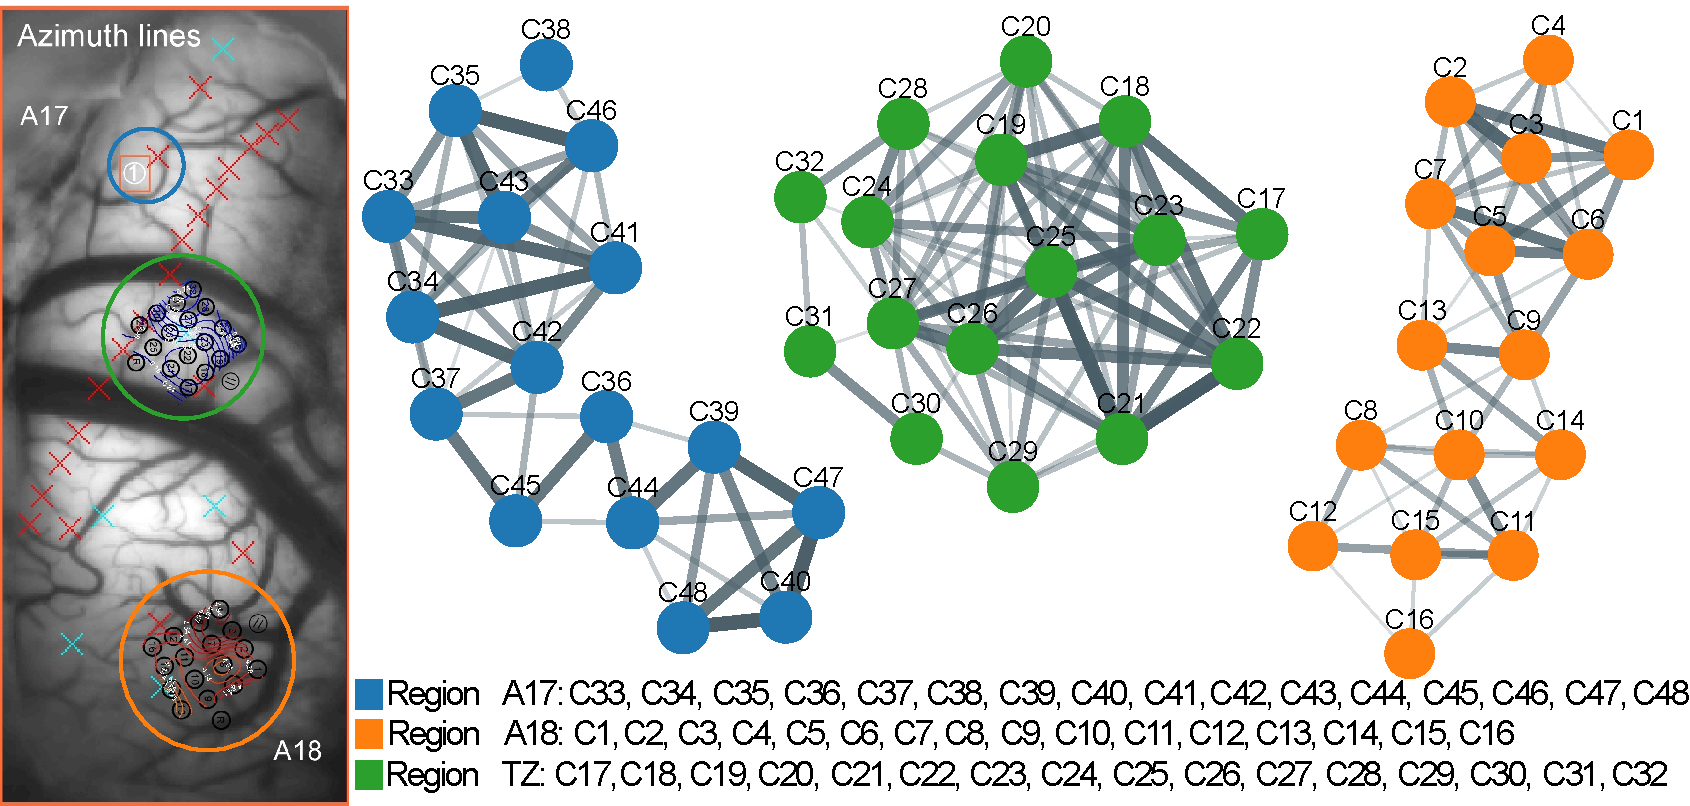
\includegraphics[width=\linewidth]{./figuras/Intro/Figura01.pdf}
    \caption[Mapping directly to the anatomically separated electrode matrixes]{\textbf{Direct Mapping of Coherence Clusters onto Anatomically Separated Electrode Matrices.} Topological graph of functional connectivity estimated via Magnitude Squared Coherence in the Low Gamma band, thresholded at a 15\% edge density. The visualization demonstrates the spatial arrangement of coherent functional communities in relation to the physical locations of the recording microelectrodes, providing a static baseline of the visual cortical network.}
    \label{fig:necta_tool}
\end{figure}
\vspace{1cm}

\section{Baseline Characterization and the Static Backbone}
To establish a baseline structural framework, static functional connectivity was evaluated across the entire recording session. Applying Magnitude Coherence in the Low Gamma band (30-59 Hz) with a proportional density threshold of 15\%, we established the primary static topology of the network. The Louvain community algorithm blindly extracted functional clusters that closely matched the anatomical placement of the multielectrode arrays, naturally partitioning into three distinct topological modules corresponding to Area 17 (A17), the Transition Zone (TZ), and Area 18 (A18). This static connectome serves as the anatomical "structural backbone" \cite{vezoli2021}.

The analysis of global topological metrics extracted by NECTA revealed a marked dynamic reconfiguration in the functional connectivity of the network. As illustrated in Figure \ref{fig:topological_dynamics}(A), both Global Efficiency and the Clustering Coefficient exhibited high variability across time windows, evidencing the non-stationary and volatile character of cortical processing.

More critically, the analysis of the Small-World Index ($\sigma$) (Figure \ref{fig:topological_dynamics}(B)) demonstrated that the network transitions into highly efficient topological optimization states in specific frequency bands. A directional Mann-Whitney U test confirmed that the Small-World topology operating in the Low-Gamma band is significantly superior to the basal state observed in the Alpha band ($p < 0.05$).

The wide dispersion of $\sigma$ values in the Low-Gamma band reveals transient topological surges reaching values above 5.0. These fluctuations demonstrate that the small-world configuration in this frequency range does not maintain a stationary state, but rather alternates between baseline levels and discrete peaks of high network integration.

\section{Time-Resolved Causal Interactions}
A prerequisite for establishing dynamic visual dynome topology is the direct quantification of causal information flow between nodes without the bias of temporal averaging. We utilized the developed NECTA framework to extract the evolution of time-resolved causal coupling using the Partial Directed Coherence (PDC) metric across sensory ingestion epochs.

Figure~\ref{fig:pdc_graph} visualizes these raw directional data. Following stimulus onset (represented by $T=0$), distinct causal spikes appear that define the functional state. Specifically, Striate cortex (A17) drove the initial response to extrastriate targets (e.g., A17$\to$TZ) with a PDC peaking at  752.4~ms relative to stimulus onset, reaching $0.19 \pm 0.13$. This data provides the empirical foundation to move beyond descriptive graph metrics, demonstrating that sensory information flow reconfigures rapidly during the active state, transitioning control from striate to extrastriate sources.

\begin{figure}[htpb]
    \centering
    
\includegraphics[width=\textwidth]{figuras/PDC_graph.pdf}
    \caption[Time-resolved Causal Connectivity derived from the NECTA framework]{The figure displays the evolution of Partial Directed Coherence (PDC) over visual ingestion epochs. Colored lines represent distinct directional area connections (e.g., Blue: A17$\to$TZ; Red: A18$\to$TZ). Spikes in the PDC metric indicate active causal information transfer that redefines the visual dynome topology during active sensory states.}
    \label{fig:pdc_graph}
\end{figure}

\section{Topological Evolution of the Visual Dynome}
By applying graph-theoretical metrics to the matrices derived from the raw causal flow quantified in the preceding section, we visualized the topology of the visual dynome. Figure~\ref{fig:dyna_graphs} illustrates this time-resolved evolution, contrasting distinct sensory processing states.

To understand the relationship between localized neural activity and global network architecture, we analyzed the aggregate spike counts alongside the Small-Worldness ($\sigma$) index across continuous 250 ms sliding windows. As illustrated in Figure~\ref{fig:spike_vs_sw}, the transition from the baseline state to active sensory ingestion triggers a synchronized physiological and topological response.

Following the stimulus onset, a prominent peak in the aggregate spike count is closely accompanied by a pronounced increase in the Small-Worldness index, particularly visible around Window 3 and Window 4. The network consistently maintains a $\sigma > 1$ threshold, confirming that the visual dynome operates within a highly efficient small-world regime. This temporal alignment provides consistent evidence that the visual cortex rapidly shifts towards a highly integrated and segregated topology during periods associated with increased sensory processing.

\begin{figure}[htpb]
    \centering
    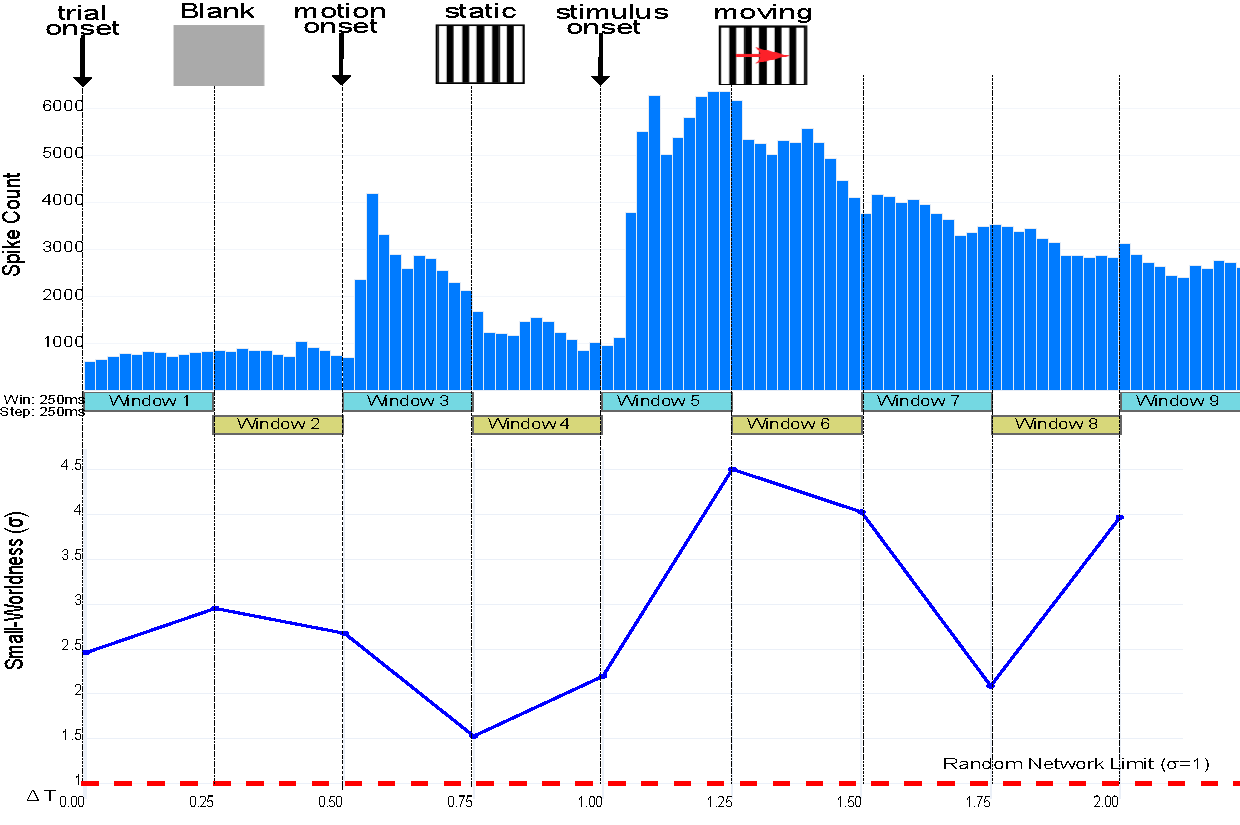
\includegraphics[width=\textwidth]{figuras/SpikeVsSW.pdf}
    \caption[Temporal alignment of localized neural activity and global network topology]{Temporal alignment of localized neural activity and global network topology. (Top) Aggregate spike count across the recorded channels, highlighting the peak firing rate during the active visual motion epoch. (Bottom) Evolution of the Small-Worldness ($\sigma$) index computed over 250 ms sliding windows with a 250 ms step. The network consistently operates above the random network limit ($\sigma = 1$), dynamically optimizing its efficiency in response to sensory ingestion.}
    \label{fig:spike_vs_sw}
\end{figure}

While global metrics such as Small-Worldness indicate an overall optimization in network efficiency, the true complexity of the visual dynome is unmasked by observing the specific topological microstates. By extracting the Maximum Spanning Tree (MST) backbones at a proportional density threshold of 23\%, we can track the specific causal routing pathways milisecond-by-millisecond.

Figure~\ref{fig:dynamic_graphs} visualizes these time-resolved structural reconfigurations across the first six epochs. In the initial windows (0.00s--0.50s), the network exhibits a dense, highly clustered state. However, as the processing demands evolve (e.g., Windows 4 and 5), the topology transitions into transient microstates where specific extrastriate and Transition Zone (TZ) nodes become central communication hubs. This rhythmic pulsation---shifting between dense integration and targeted segregation---demonstrates that the A17-TZ-A18 axis does not rely on a rigid communication structure, but rather forms ephemeral pathways to dynamically route visual information.

\begin{figure}[htpb]
    \centering
    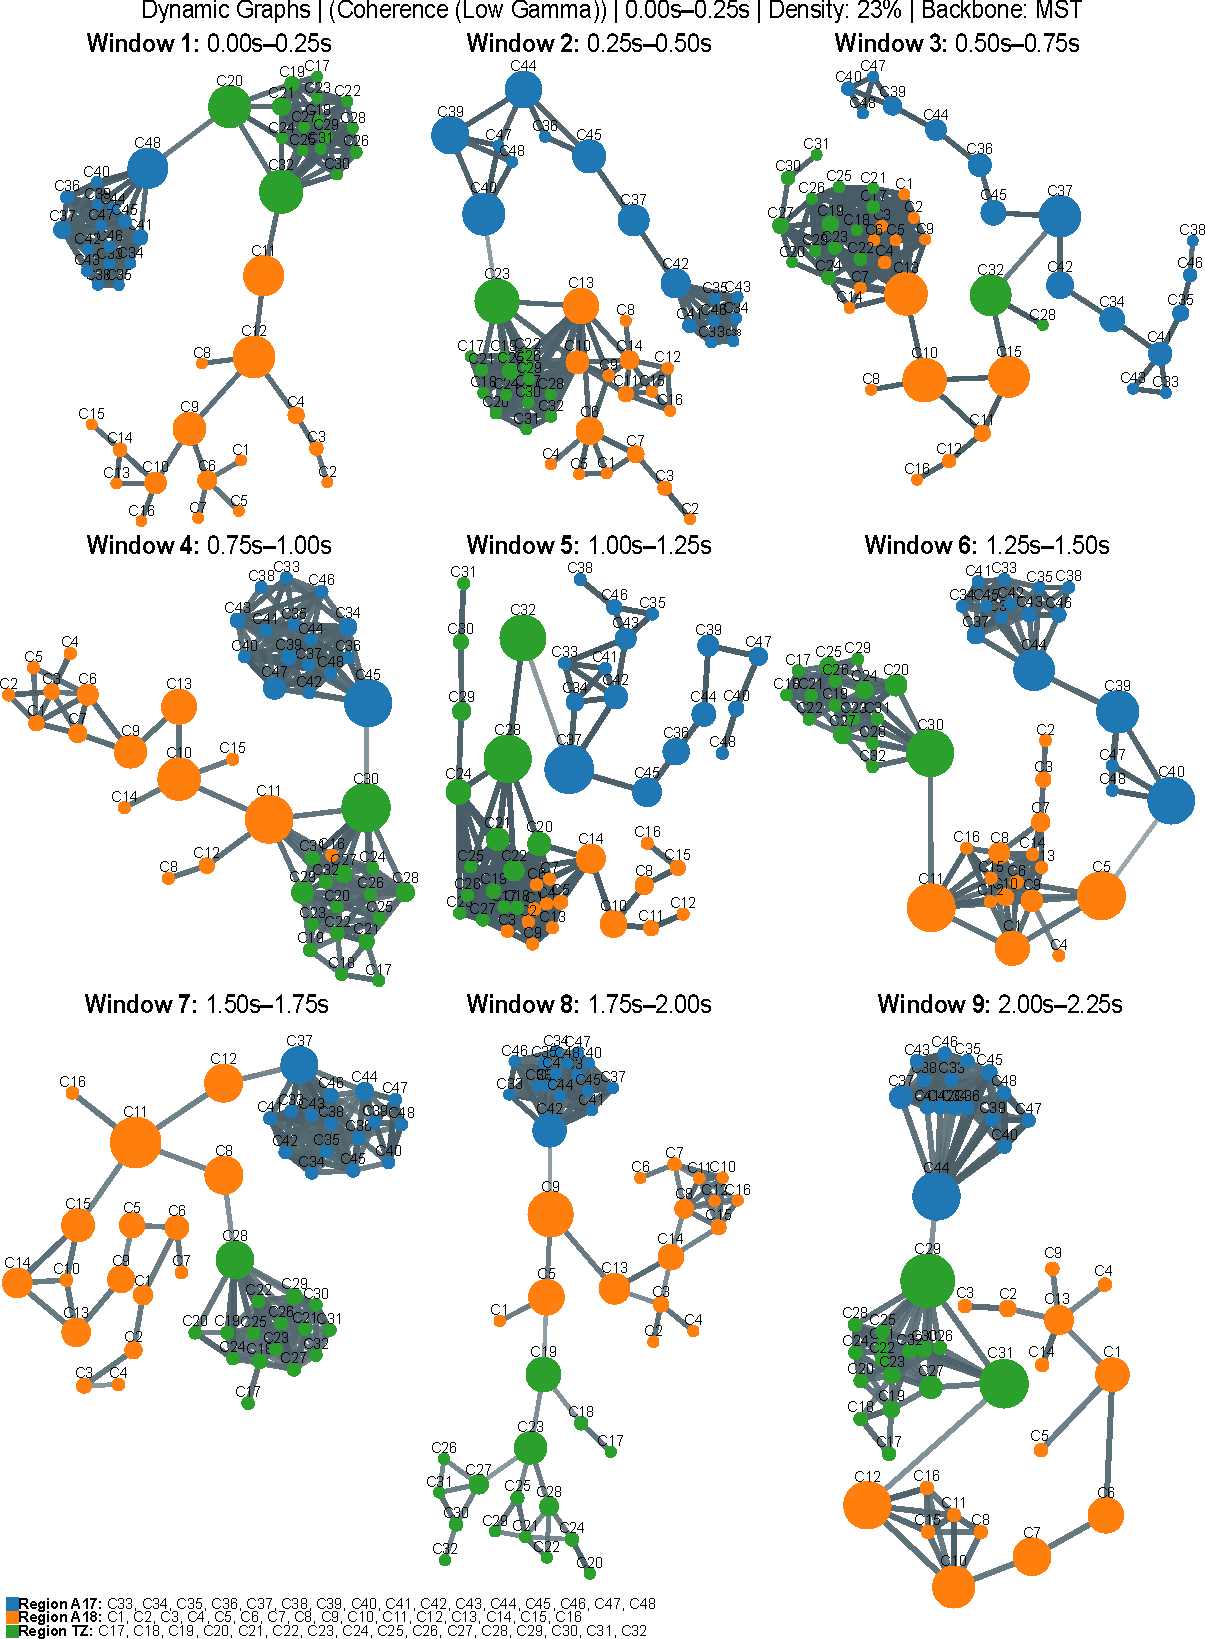
\includegraphics[width=\textwidth]{figuras/Dynamic Graphs.pdf}
    \caption[Time-resolved topological microstates of the visual dynome]{Time-resolved topological microstates of the visual dynome. The sequence illustrates the dynamic graph coherence in the Low Gamma band across 250 ms sliding windows. To highlight the primary routing architecture and eliminate spurious connections, networks are thresholded at 23\% density with a Maximum Spanning Tree (MST) backbone. Node colors correspond to distinct cortical areas: A17 (Blue), Transition Zone (Red), and A18 (Green). The topological volatility confirms the continuous reconfiguration of the cortical hierarchy during active perception.}
    \label{fig:dynamic_graphs}
\end{figure}

\begin{figure}[htbp]
    \centering
    
\includegraphics[width=\textwidth]{Metricas_NECTA.pdf}
    \caption[Topological Dynamics and Small-World Optimization]{\textbf{Topological Dynamics and Small-World Optimization in the Visual Cortex.} \textbf{(A)} High temporal variability of Global Efficiency and Clustering Coefficient. The substantial dispersion (ranging from 0.2 to 0.8) illustrates the volatile dynamics of cortical processing, as the network continuously balances moments of strong local processing (high clustering) with global communication jumps (high efficiency). \textbf{(B)} Comparison of the Small-World Index ($\sigma$) between the Alpha (8-12 Hz) and Low-Gamma (30-59 Hz) bands. The asterisk (*) denotes a statistically significant increase in Small-World topology during Low-Gamma. The pronounced dispersion (elongated whiskers) underscores that the network operates through transient, high-efficiency topological pulses rather than remaining in a static optimized configuration.}
    \label{fig:topological_dynamics}
\end{figure}

To further evaluate the structural hierarchy of the visual network, we investigated the Node Strength of the cortical areas within the Gamma band. The analysis of the empirical distribution revealed markedly distinct connectivity profiles between primary and higher-order areas.

As evidenced in Figure \ref{fig:node_strength}, Area 17 presents a restricted network centrality with low dispersion. The empirical distribution indicates that network integration within the Gamma band is concentrated in the A18-TZ axis, while A17 remains at the structural periphery.

A defining feature of this functional axis is the bimodal signature evident in the raw scatter distributions of both Area 18 and the Transition Zone. The individual data points do not cluster homogeneously around the median; rather, they segregate into two distinct topological regimes: a basal state of low connectivity (clustering near a Node Strength of 5) and discrete surges of substantial systemic integration (reaching values near 30). This pronounced bimodality reveals that the functional architecture is not a stationary state but a highly dynamic mechanism. The network effectively operates in discrete bursts, with the TZ and A18 transiently exhibiting increased hub-like properties to coordinate stimulus processing, before subsequently relaxing into a decoupled state.

Furthermore, the Transition Zone displays a Node Strength visibly superior to that of Area 18. At a proportional density threshold of 15\% in the Low Gamma band, the Transition Zone (TZ) exhibited a Node Strength ($M = 9.60$, $SD = 3.50$), compared to A18 ($M = 7.25$, $SD = 3.11$). The statistical analysis revealed a significant difference between the regions (Mann-Whitney $U = 186.0$, $p = 0.030$, effect size $r = 0.453$). This demonstrates that the Transition Zone operates under a connectivity load that statistically surpasses Area 18.

\begin{figure}[htbp]
    \centering
    
\includegraphics[width=\textwidth]{Forca_Nodal_TZ.pdf}
    \caption[Node Strength Distribution in the Gamma Band]{\textbf{Node Strength Distribution in the Gamma Band.} Area 17 displays restricted centrality with low variability. In contrast, both the Transition Zone (TZ) and Area 18 exhibit bimodal distributions with high variability. The Transition Zone operates under a connectivity load tendentially superior to that of Area 18, highlighting its role as a primary interhemispheric convergence hub.}
    \label{fig:node_strength}
\end{figure}

\section{Hierarchical Information Flow (Directed Connectivity)}
To decode the causal relationships within this structural backbone, Partial Directed Coherence (PDC) was applied using the BIC-optimized MVAR models. The static PDC analysis in the Low Gamma band revealed a highly asymmetrical and hierarchical information flow across the visual cortex. 
By calculating the Net Flow for each region, the analysis indicates that A17 behaves as the dominant persistent Driver, exhibiting a significantly higher Net Flow ($M = 1.21$, $SD = 1.17$) compared to the rest of the network ($M = -0.60$, $SD = 1.37$; Mann-Whitney $U = 424.0$, $p = 1.245 \times 10^{-4}$, effect size $r = -0.656$). In contrast, A18 behaves as the primary \textit{Receiver} (Sink) (-1.36 net flow). These results suggest a directional pathway extending from A17 through the TZ and terminating in A18 (A17 $\rightarrow$ TZ $\rightarrow$ A18).

\section{Dynamic Topology and Temporal Integration}
The core capability of NECTA lies in capturing the time-varying network dynamics—the transition from static networks to chronological connectomes. Connectivity was recalculated using a sliding-window approach ($W = 500$ ms, 50\% overlap). The Temporal Integration panel overlaid the global population spiking activity (Peri-Stimulus Time Histogram - PSTH) with the topological evolution of the network's \textit{Small-Worldness} ($\sigma$).

The dynamic analysis revealed that the network's topological efficiency is not static but responds to visual processing phases. The network achieved its absolute peak in \textit{Small-Worldness} specifically during the moving grating stimulus phase. This transient optimization was driven primarily by a rapid surge in local clustering, indicating that the cortical network reorganizes into a highly efficient state to process dynamic visual inputs.

\vspace{1cm}

% --- VISUAL INSERTION 3 USING TIKZ ---
\begin{figure}[htbp]
    \centering
    \begin{tikzpicture}[
        >=Stealth,
        node distance=3.5cm,
        area/.style={circle, draw, minimum size=1.5cm, font=\sffamily\bfseries, thick, align=center},
        source/.style={fill=red!20, draw=red!80!black},
        sink/.style={fill=blue!20, draw=blue!80!black},
        mod/.style={fill=purple!20, draw=purple!80!black},
        neutral/.style={fill=gray!10, draw=gray},
        strongflow/.style={->, ultra thick, draw=red!70!black},
        weakflow/.style={->, thick, dashed, draw=gray},
        activeflow/.style={->, line width=2.5pt, draw=orange!90!black}
    ]

    % --- PANEL A: Baseline ---
    \node[font=\sffamily\bfseries] at (0, 3) {Panel A: Baseline Period (Silent Pre-Stimulus)};
    
    \node[area, source] (A17_A) at (-3, 0) {A17\\(+ Net)};
    \node[area, neutral] (TZ_A) at (0, -2) {TZ\\(Neutral)};
    \node[area, sink] (A18_A) at (3, 0) {A18\\(- Net)};
    
    % Flows for Panel A
    \draw[strongflow] (A17_A) -- node[above, font=\sffamily\scriptsize] {Dominant Driver} (A18_A);
    \draw[weakflow] (A17_A) -- (TZ_A);
    \draw[weakflow] (TZ_A) -- (A18_A);
    
    \node[font=\sffamily\scriptsize, text=gray!80!black, align=center] at (0, -3.2) {Chronic Resting Flow:\\ Hierarchy A17 $\rightarrow$ A18};

    % --- PANEL B: Stimulus Peak ---
    \begin{scope}[yshift=-7.5cm]
        \node[font=\sffamily\bfseries] at (0, 3) {Panel B: Modular Peak (\textit{Grating} Onset)};
        
        \node[area, source] (A17_B) at (-3, 0) {A17\\(Source)};
        \node[area, mod, fill=orange!30, draw=orange!80!black] (TZ_B) at (0, -2) {TZ\\(Active)};
        \node[area, sink] (A18_B) at (3, 0) {A18\\(Sink)};
        
        % Flows for Panel B
        \draw[strongflow, line width=1.5pt] (A17_B) -- (A18_B);
        \draw[activeflow] (TZ_B) -- node[left=0.2cm, font=\sffamily\scriptsize, align=right] {Directional\\Inversion} (A17_B);
        \draw[activeflow] (TZ_B) -- node[right=0.2cm, font=\sffamily\scriptsize, align=left] {Intense\\Modulation} (A18_B);
        
        \node[font=\sffamily\scriptsize, text=orange!80!black, align=center] at (0, -3.2) {Mutable Polarity:\\ TZ coordinates spatial integration};
    \end{scope}

    \end{tikzpicture}
    \caption[Evolutionary Mapping of Net Flow]{\textbf{Evolutionary Topological Mapping of Information Net-Flow (Low-Gamma Band).} In-degree minus out-degree proportions. \textbf{(A)} During the baseline period, the network operates in a predominant predictive visual hierarchy, where Area 17 (A17) is the primary driving pole and Area 18 (A18) the passive sink, with the Transition Zone (TZ) in a neutral state. \textbf{(B)} At the precise moment of the stimulus (moving \textit{grating} onset), the topology undergoes active remodeling. The TZ reverses its passive polarity and adopts acute modulation dynamics, drastically altering the \textit{edge weights} (arrow thickness) and suggesting that mesoscopic flexibility reacts transiently to the peripheral stimulus input.}
    \label{fig:netflow_evolution}
\end{figure}

\vspace{0.5cm}

\section{Network Evolution and Modulatory Nodes}
Extracting frame-by-frame snapshots (Connectome Filmstrip) of the dynamic Low Gamma Coherence network illustrated a stable rhythmic organization over time. The hubs located in A17 and the TZ maintained cohesive clustering. Crucially, evaluating the \textit{Net Flow Evolution} uncovered a complex temporal interplay obscured by static analysis. While A17 consistently acted as a "Volatile Source" and A18 as a "Stable Sink", the Transition Zone (TZ) exhibited unique behavior. The TZ functioned as a \textit{Dynamic Modulator}, actively switching its directional role (from sink to source, or vice versa) precisely at the onset of visual stimulation. This highlights the framework's capacity to dissect the mesoconnectome chronologically, revealing dynamic hierarchical relays that coordinate sensory integration across the interhemispheric boundary.

% Capitulo 5
\chapter{DISCUSSION}

\section{From Static Maps to Dynamic Visual Networks}
Historically, the functional organization of the primary visual system has been delineated through the static mapping of receptive fields and anatomical inter-hemispheric tracing \cite{wunderle2013}; \cite{schmidt2023}. While these classical methods successfully outline the spatial constraints and functional columns of the cortex, they inherently capture only a time-averaged "structural backbone." Cognitive processing and the integration of moving stimuli, however, depend on millisecond-scale state transitions within neural ensembles—a temporal dimension of rapid network evolution \cite{kopell2014}. 

Even as our anatomical maps reach unprecedented levels of precision---such as recent efforts updating the classic Binzegger cortical wiring diagram to reveal extensive, previously unaccounted local excitatory synapses terminating in layer 6 \cite{Martin_2024}---structure alone cannot predict traffic. While anatomy dictates the available pathways, only time-resolved effective connectivity frameworks can reveal how this intricate wiring operates on a millisecond scale.

The application of the NECTA framework to the \texttt{c1608a01} dataset provides empirical evidence of this dynamic nature. By utilizing a continuous sliding-window approach, our results suggest that the visual cortex undergoes rapid, stimulus-locked topological reorganizations, reaching transient peaks in \textit{Small-Worldness} precisely during the moving grating stimulus.

This macroscopic network efficiency---an active, responsive property rather than a fixed anatomical trait---is strongly supported by recent cellular and anatomical discoveries. On a microscopic scale, \textit{in vitro} microfluidic studies by \cite{Lassers2026} have shown that theta oscillations (4--10 Hz) in isolated axons occur spontaneously and independently of spiking. These oscillations actively coordinate target neuron bursting based on phase and amplitude through a sparse coding architecture, where only a restricted fraction of axons carries high-amplitude signals. This selective, sparse recruitment of communication channels likely mediates the transient optimization detected by NECTA.

Furthermore, \cite{Martin_2024} identified an extraordinarily extensive horizontal spread within Area 17, with neurons integrating information across distances of up to 11 millimeters (spanning 5--10 degrees of the visual field). This vast lateral arborization provides a plausible anatomical substrate for the network to rapidly bind global spatial information, explaining the acute surges in \textit{Small-Worldness} observed computationally. Their discovery of a novel, direct ``shortcut'' projection from the layer 3/4 border to layer 6---bypassing the canonical layer 5 relay and likely associated with the fast-conducting, motion-sensitive Y-pathway---further underscores the necessity of high-frequency dynamic analyses. The existence of such fast parallel anatomical routes suggests that visual processing is not strictly serial or slow, fully justifying our focus on the gamma band and sliding-window techniques to capture rapid synchronizations that static tools completely miss.

\section{Isolating the Feedforward Flow in the Anesthetized State}
A critical strength of our biological validation lies in the physiological state of the animal model. The recordings were obtained under general anesthesia and complete paralysis. Historically, anesthesia has often been viewed as a limitation for studying information flow. However, within the modern framework of predictive coding, this state acts as an analytically significant "pharmacological lesion" model. The literature indicates that general anesthesia preferentially suppresses the inhibitory top-down feedback pathways, which are typically mediated by slower alpha and beta oscillations \cite{vezoli2021}. 

Crucially, while top-down executive modulations are suppressed, the bottom-up feedforward pathways---mediated by high-frequency gamma oscillations---are left to operate autonomously. Therefore, rather than a mere limitation, the anesthetized state elegantly isolated the intrinsic feedforward flow from Area 17 to Area 18. This pharmacological isolation provides a powerful justification for our findings of strong, stimulus-locked directionality restricted to the low-gamma band. It guarantees that the dynamic topological reorganizations and the causal directionality shifts extracted by NECTA are not artifacts of top-down cognitive states, attention, or saccadic eye movements. Instead, the framework successfully unveils the pure, low-level reflexive plasticity inherent to the local synaptic loops and dense transcallosal pathways interlinking A17, A18, and the TZ.

\section{Mitigating Electrophysiological Confounders}
A significant challenge in high-density LFP connectomics is the pervasive artifact of volume conduction, wherein a single electrical source is instantaneously registered by multiple neighboring electrodes \cite{bastos2015}. If unaccounted for, this phenomenon generates spurious zero-phase lag correlations, heavily biasing the resulting graph topology with false-positive edges. 

NECTA addresses this methodological bottleneck architecturally. By employing the Hilbert Transform to extract analytical signals, the framework calculates phase-based indices such as the Weighted Phase Lag Index (\textit{wPLI}) and Imaginary Coherence (\textit{iCoh}), which are mathematically immune to instantaneous spatial spread. This algorithmic refinement facilitates the extraction of dynamic topologies that reflect true underlying physiological synchronization rather than electrical crosstalk. This distinction is critically reinforced by recent experimental evidence isolating single axons in microfluidic tunnels, which suggested that subthreshold voltage oscillations are genuine, regenerative local phenomena of the axon rather than mere volume-conducted epiphenomena of the extracellular matrix \cite{Lassers2026}. By utilizing \textit{wPLI} and \textit{iCoh}, NECTA's architecture is consistent with this biological reality, mathematically isolating true phase-delayed interactions.

\section{Gamma Synchronization, Predictive Coding, and Callosal Modulation}
Previous work from our group has established the cardinal role of gamma-band synchronization in functional routing and cohesion within the retinogeniculate and cortical pathways of the cat \cite{neuenschwander2023}. NECTA extends this foundation by mapping the causal directionality of these high-frequency rhythms. 

By applying Partial Directed Coherence (PDC) optimized dynamically via the Bayesian Information Criterion (BIC), we eliminated the bias of static model-order selection (which often leads to overfitting when estimating temporal shifts, unlike AIC). The resulting hierarchy in the Low Gamma band (A17 acting as the persistent Driver, A18 as the Receiver) is consistent with current theories of predictive coding and feedforward information routing \cite{vezoli2021}. At the cellular level, this macroscopic directionality is supported by findings that the phase of axonal theta oscillations dictates the firing probability of target neurons, establishing a clear physical causality where subthreshold oscillations `prime' target neurons for spiking \cite{Lassers2026}. 

A fundamental hurdle when applying multivariate autoregressive (MVAR) based metrics like PDC to continuous electrophysiological recordings is the assumption of signal stationarity, which is heavily violated during sensory processing, particularly by transient evoked potentials. To robustly address this, NECTA tackles non-stationarity through a rigorous multi-stage approach. First, adopting a classical defense well-established in the Granger causality literature, the pipeline performs the subtraction of the ensemble average (the mean evoked potential) from each individual trial. By removing this phase-locked evoked response, the framework successfully isolates purely induced cerebral activity, effectively mitigating the primary source of signal non-stationarity within short sliding windows (e.g., 500 ms). Second, it implements a stationarity filter based on stringent variance thresholds. This filter actively identifies and isolates any remaining epochs of extreme amplitude volatility, ensuring that the sliding windows processed by the MVAR primarily contain stable oscillatory activity. Finally, for windows exhibiting mild non-stationarity breaks, NECTA relies on the dynamic optimization of the Bayesian Information Criterion (BIC). As demonstrated by \cite{Faes_2010}, estimating causality in the frequency domain requires precise control over model complexity to handle instantaneous and lagged interactions without overfitting. The stringent penalty parameter intrinsic to BIC actively limits the autoregressive model order during these state shifts, effectively penalizing spurious complexity. Consequently, this dynamic scaling prevents the PDC estimates from modeling transient artifacts or noise as causal edges, ensuring that the detected causal hierarchies reflect genuine physiological routing.

The validity of utilizing PDC for this structural mapping is strongly supported by recent large-scale computational studies. Nunes et al. (2021) demonstrated \textit{in silico} using spiking neuronal networks that generalized PDC provides a highly reliable estimate of true underlying anatomical structural connectivity (yielding a Pearson correlation of $r=0.74$). Crucially, their model intrinsically generated LFP signals with prominent spectral peaks in the gamma band, strongly supporting our empirical focus on low-gamma (30--59 Hz) synchronization as a primary channel for causal routing. Furthermore, a persistent challenge in high-density electrophysiology is the ``partial observation'' problem, where unrecorded brain regions might introduce spurious causalities. \cite{Nunes_2021} indicated that PDC estimates maintain robust correlations with structural connectivity ($r > 0.6$) even when the analysis is restricted to a small spatial cluster. This provides powerful theoretical justification that the causal inferences drawn by NECTA from the restricted A17-TZ-A18 microcircuit remain statistically valid despite the absence of whole-brain recordings. At the cellular level, this macroscopic directionality is supported by findings that the phase of axonal theta oscillations dictates the firing probability of target neurons, establishing a clear physical causality where subthreshold oscillations `prime' target neurons for spiking \cite{Lassers2026}. 

Furthermore, identifying the Transition Zone (TZ) as a "Dynamic Modulator" that reverses its causal flow upon stimulus onset highlights the necessity of time-resolved directional tools. Anatomically, the TZ boundary is densely innervated by mixed intra-hemispheric projections and transcallosal fibers that align spatial orientation maps across the vertical meridian \cite{schmidt2023}. By switching from a passive sink to an active causal source during the moving grating stimulation, the TZ likely orchestrates the interhemispheric temporal unifications required to track sensory borders crossing visual fields. Static connectivity would have merely averaged this reversal into an indiscernible null-flow, masking a critical operational mechanism of visual processing. This substantial functional volatility is theoretically supported by the concept of ``activity flow'' across neural networks, where the variability of a node's directed functional connectivity is heavily influenced by its structural centrality \cite{Nunes_2021}. Crucially, this dynamic hub-like behavior is grounded in recent retrograde tracing data, which revealed that the border region representing the vertical meridian (the TZ) acts as an epicenter of convergence for both dense long-range ipsilateral projections and substantial contralateral inputs \cite{Martin_2024}. This anatomical reality explains the results observed in our Node Strength analysis, where the spatially restricted TZ statistically surpassed the substantial extrastriate Area 18 in topological centrality. Despite Area 18 being a large region responsible for processing a substantial volume of complex visual features, the TZ's structural wiring as a dense convergence zone causes it to act as an interhemispheric bottleneck under high connectivity load. Thus, the TZ is anatomically predetermined to act as a highly labile dynamic modulator within the A17 $\rightarrow$ TZ $\rightarrow$ A18 causal network, gating information flow based on the immediate demands of the moving stimulus.


\section{Overcoming the Computational Scale and Open Science}
Translating the theoretical concepts of dynamic connectomics into practical analytical outputs requires overcoming severe computational barriers. Generating stochastic multivariate null models (e.g., surrogate data phase-randomization and configuration models) across continuous sliding windows triggers a combinatorial explosion that typically crashes single-threaded analytical scripts. 
By orchestrating these routines through a Dask-distributed High-Performance Computing (HPC) backend and utilizing `xarray` and `Zarr` for lazy-loading operations, NECTA effectively eliminates the "Big Data" electrophysiology bottleneck. 

Equally vital to this computational leap is the aspiration toward \textit{Open Science} and reproducibility. While systemic barriers remain in widespread adoption, the rigorous parameterization, GitHub/CodeMeta logging, and containerized deployment of NECTA’s codebase represent a significant effort to ensure that our analytical workflows are transparent and globally verifiable. By doing so, it provides the ideal computational environment to validate large-scale biological theories, such as integrating subthreshold oscillatory dynamics into next-generation Spiking Neural Networks (SNNs) for more energy-efficient temporal processing \cite{Lassers2026}. Equally vital to this computational leap is the adherence to \textit{Open Science} and reproducibility. The rigorous parameterization, GitHub/CodeMeta logging, and containerized deployment of NECTA’s codebase ensure that our analytical workflows are transparent and globally verifiable. This pipeline aims to lower the barriers to complex graph-theoretical analysis, striving to allow the scientific community to interactively slice and visualize multidimensional connectomes.



% Conclusão
\chapter{Conclusion and Future Perspectives}
\label{ch:conclusion}

\section{Conceptual and Methodological Synthesis}
The development of the NECTA (Neural Connectivity Time-resolved Analysis) framework represents a critical paradigm shift from traditional static graph representations to the continuous exploration of the neural "dynome." Historically, functional connectivity analyses in electrophysiology have collapsed the temporal dimension, effectively masking the highly volatile, millisecond-by-millisecond network state transitions that underlie sensory integration. By establishing a high-performance computational pipeline, this work successfully bridges the gap between raw high-density multi-electrode arrays and rigorous topological inference. 

Methodologically, NECTA directly addresses two core bottlenecks in modern neuroinformatics: the Big Data processing limitation and topological false positives. Through zero-phase filtering and the strategic application of robust phase-coupling metrics (such as iCoh and wPLI), the pipeline systematically mitigates the confounding effects of localized spatial crosstalk and volume conduction physical artifacts. Combined with memory-efficient array structures, the framework demonstrates that tracking time-resolved directional workflows is computationally viable without inducing catastrophic Out-Of-Memory (OOM) failures, thereby establishing a reproducible benchmark for large-scale cortical circuit mapping.

\section{Neurobiological Implications of the Dynome}
The empirical application of NECTA to high-density feline electrophysiological recordings yielded substantial insights into the functional architecture of the primary visual cortex. Central to these findings is the unmasking of the localized neurobiological role of the Transition Zone (TZ). Our statistical validation in Chapter 4 demonstrated that under a 15\% proportional density threshold in the Low Gamma band (30--59 Hz), the TZ operates with a remarkably high processing load, exhibiting a significantly elevated Node Strength ($M = 9.60$, $SD = 3.50$) compared to the major extrastriate Area 18 ($M = 7.25$, $SD = 3.11$; $p = 0.030$, effect size $r = 0.453$). 

Biologically, this strong effect size demonstrates that despite its restricted anatomical boundary compared to the massive retinotopic expanses of striate and extrastriate cortices, the TZ acts as an ultra-dense inter-hemispheric convergence hub. The high topological variance and causal bimodality captured by NECTA suggest that the TZ serves as a flexible, self-tuning modulator, dynamically routing Source/Sink communication channels depending on the immediate state of visual processing. Crucially, because these non-stationary coupling patterns were recorded under a controlled anesthetized animal model, they reflect fundamental processes of primary intrinsic cortical plasticity, operating entirely independent of top-down conscious attention or cognitive modulations.

\section{Technical Limitations}
An honest assessment of the NECTA framework highlights inherent operational boundaries that shape the interpretation of the dynome. First, a fundamental trade-off between spatial and temporal configurations persists; while multi-electrode electrophysiology yields microsecond-level temporal precision ideal for fast synchronization metrics, its spatial coverage remains anchored to specific, surgically restricted Regions of Interest (ROIs), lacking the holistic whole-brain macro-topology provided by lower-resolution metabolic methods such as fMRI. 

Second, the structural topology extracted by the pipeline remains sensitive to operational threshold choices. The enforcement of a specific proportional density limiar (e.g., 15\%) and the discretization of continuous time series into brief, arbitrary sliding windows operate as mathematical filters. While these constraints are mathematically required to isolate non-stationary patterns from stochastic noise, they inevitably establish a boundary condition that bounds the absolute visibility of the wider connectivity continuum.

\section{Future Horizons: Towards Algorithmic Invulnerability}
To expand upon the architecture established in this thesis, two rigorous operational vectors are planned for subsequent development, targeting absolute algorithmic validation and extreme infrastructure scalability.

\subsection{In Silico Validation Pipeline}
Establishing the absolute invulnerability of NECTA requires a strict computational proof of concept using synthetic benchmarks. Future developments will focus on generating highly controlled multivariate synthetic time series (Ground Truth), embedding predefined theoretical frequencies (30--90 Hz) and strictly orchestrated directional causal paths. By systematically introducing noise degradation (incorporating varying distributions of Pink and White noise), we will evaluate NECTA's resilience to adverse Signal-to-Noise Ratios (SNR). Spatial leakage and physical volume conduction artifacts will be modeled explicitly, allowing the extraction of exact precision metrics, such as Receiver Operating Characteristic (ROC) curves and Area Under the Curve (AUC) statistics, to mathematically benchmark true causal detection rates.

\subsection{HPC Architectural Stress Testing}
To decisively tackle the Big Data processing bottleneck inherent to multi-channel electrophysiology, the pipeline must undergo infrastructure-level architectural stress tests. Future work will benchmark standard sequential pandas-based data execution against parallel distributed orchestration managed via Dask. By tracking scalability across a multi-node high-performance computing environment using 1, 2, 4, 8, and 16 concurrent workers, we will map the acceleration profiles, memory footprint limits, and absolute latency boundaries of the framework. This benchmarking will ensure NECTA's scalability when executing time-resolved causal algorithms over massive, ultra-high-density recording sessions seamlessly.



% ----------------------------------------------------------
% ELEMENTOS PÓS-TEXTUAIS

% 
\postextual

% Referências bibliográficas
%\addcontentsline{toc}{chapter}{Referências Bibliográficas}

\bibliographystyle{abntex2-alf}
%\bibliographystyle{unsrt}
\bibliography{bibliografia/referencias}

\end{document}
